\documentclass[a4paper]{article}
\usepackage[letterpaper, margin=1in]{geometry} % page format
\usepackage{listings} % this package is for including code
\usepackage{graphicx} % this package is for including figures
\usepackage{amsmath}  % this package is for math and matrices
\usepackage{amsfonts} % this package is for math fonts
\usepackage{tikz} % for drawings
\usepackage{hyperref} % for urls
\usepackage{titling}
\usepackage{indentfirst}
\usepackage{dsfont}
\setlength{\parindent}{1em}

\title{\textbf{American Sign Language Detection}}
\author{Xiang Fang}
\date{\today}

\begin{document}

\maketitle

\begin{abstract}
This project explores and utilizes the application of state-of-the-art object detection models for recognizing American Sign Language (ASL) gestures. 
Through an relatively small dataset with some data augmentation techniques, we evaluate the performance of models such as YOLOv11, Faster R-CNN, and RT-DETR. Key metrics, 
including mean Average Precision 50-95 (mAP 50-95) and Intersection over Union (IoU), are explained and used to benchmark model accuracy. The findings highlight the strengths and limitations of each model, 
providing a basis for future improvements in ASL gesture detection.
\end{abstract}

\tableofcontents
\newpage

\section{Introduction}

Object detection is a cornerstone of computer vision, involving the identification and localization of objects within images or video streams. Unlike traditional classification tasks that label an image as a whole, 
object detection not only identifies objects but also delineates their positions using bounding boxes. This dual capability makes it invaluable in applications ranging from autonomous vehicles to medical imaging and surveillance.

At its core, object detection combines elements of classification and regression. Classification determines the category of an object, while regression predicts the coordinates of the bounding box enclosing the object. 
Modern object detection techniques often employ deep learning models, leveraging convolutional neural networks (CNNs) for feature extraction and prediction.

% Insert Object Detection Diagram
\begin{figure}[h!]
    \centering
    % Add your image file name in the placeholder below
    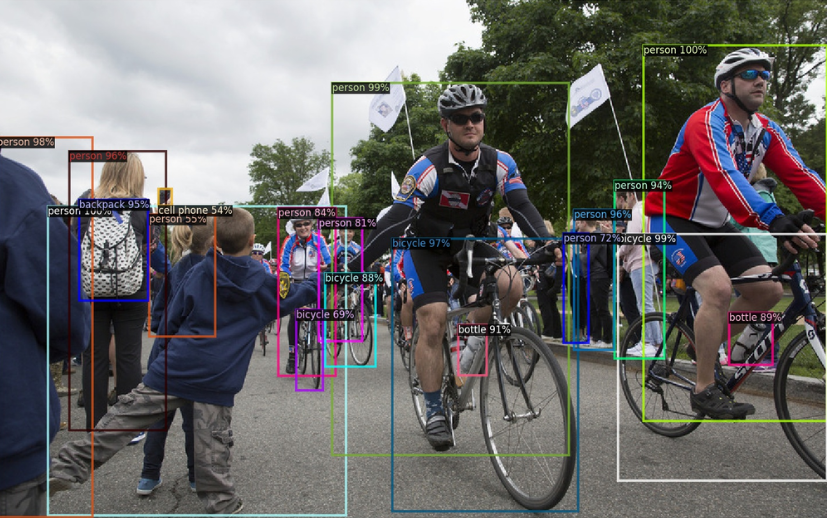
\includegraphics[width=0.8\textwidth]{./images/detectron.png}
    \caption{Objection Detection output from detectron2}
    \label{fig:object_detection}
\end{figure}
    Object detection is a critical task in computer vision, aiming to detect and locate objects of interest in images or videos. In this project, we focus on detecting American Sign Language (ASL) gestures, 
    which involve recognizing specific hand signs corresponding to letters or words. The primary objective is to improve the accuracy and robustness of ASL detection using state-of-the-art models.

\subsection{Problem Statement}
ASL detection involves identifying the position and boundaries of hand gestures and classifying them into different categories. The task poses challenges due to several inherent complexities:
\begin{itemize}
    \item \textbf{Variability in Gestures:} Hand gestures for ASL vary significantly in shape, orientation, and motion, making consistent detection challenging.
    \item \textbf{Lighting Conditions:} Variations in lighting, such as shadows or glare, can affect the visibility and clarity of gestures.
    \item \textbf{Background Complexity:} The presence of cluttered or dynamic backgrounds complicates the isolation of hand gestures.
    \item \textbf{Inter-Class Similarity:} Some ASL gestures are visually similar, leading to potential misclassifications.
    \item \textbf{Real-Time Requirements:} Ensuring low-latency detection for real-time applications adds an additional layer of complexity.
\end{itemize}

Addressing these challenges requires robust models capable of handling diverse input conditions and providing high precision and recall rates across all ASL gestures.

\section{Background and Related Work}
Object detection has evolved from basic classification tasks to advanced techniques like segmentation and multimodal models. Key approaches include:
\begin{itemize}
    \item \textbf{Anchor-Based Models:} Anchor-based models rely on predefined bounding boxes (anchors) that are placed across the image grid at different scales and aspect ratios. Each anchor is matched with the closest ground truth object based on overlap, typically measured using the Intersection over Union (IoU) metric. These models predict adjustments to the anchors to better fit the detected objects. Anchor-based methods, like Faster R-CNN and YOLOv3/v4, are computationally intensive due to the large number of anchors generated but excel at handling objects of varying sizes and aspect ratios.
    \item \textbf{Anchor-Free Models:} Unlike anchor-based methods, anchor-free models directly predict object centers or key points and regress the bounding box coordinates. This approach reduces the computational overhead of generating and processing anchors. Models like YOLOv8 and DETR exemplify this approach, focusing on the simplicity and efficiency of detection while maintaining high accuracy. Anchor-free methods are particularly advantageous for detecting objects with extreme aspect ratios or under complex scenes. Predict object centers or key points directly (e.g., YOLOv8, DETR).
    \item \textbf{One-Stage Detectors:} These models perform detection in a single step, combining region proposal and classification into a unified architecture. By predicting bounding boxes and class probabilities directly from feature maps, one-stage detectors like YOLO and RetinaNet are optimized for speed, making them suitable for real-time applications. Although one-stage detectors are faster, they may trade off some accuracy when compared to two-stage methods, particularly for small or overlapping objects.
    \item \textbf{Two-Stage Detectors:} Two-stage detectors divide the detection process into two steps: a Region Proposal Network (RPN) generates candidate object regions, and a second stage classifies these regions and refines their bounding box coordinates. Faster R-CNN and Mask R-CNN are notable examples. Two-stage detectors are more computationally intensive but achieve higher accuracy, particularly for complex scenes with small or closely packed objects. Their modular design allows for flexibility in feature extraction and proposal refinement. Split detection into region proposal and refinement stages (e.g., Faster R-CNN).
\end{itemize}

\subsection{Related Models}
\begin{itemize}
    \item \textbf{YOLO:} Single-stage detector that divides images into grids for real-time detection. YOLO has evolved through multiple versions, including significant improvements in accuracy and speed. It uses a backbone for feature extraction, a neck for feature aggregation, and a head for generating predictions. Non-maximum suppression ensures unique detections. \cite{1}
    \item \textbf{Faster R-CNN:} Two-stage detector with high accuracy for small and overlapping objects. Its region proposal network (RPN) generates candidate object regions, which are refined and classified in the second stage. The model leverages ROI pooling and fully connected layers for precise detection. \cite{3}
    \item \textbf{DETR:} Transformer-based model with anchor-free query detection. DETR uses an encoder-decoder structure, where the encoder processes image features and the decoder refines object queries. It employs cross-scale and intra-scale feature interactions for accurate predictions. \cite{4}
\end{itemize}

\newpage
\section{Dataset and Preprocessing}
\subsection{Dataset Details}
The dataset \cite{5} comprises 1,728 original images, split into training (1,512), validation (144), and test (72) sets. Images are resized to $384\times384$ pixels.

\subsection{Data Augmentation}
To improve model generalization, over 20 augmentation techniques were employed, expanding the training set to 15,110 images and the validation set to 2,801. Techniques include:
\begin{itemize}
    \item \textbf{Rotation, Flip:} Simulates different orientations.
    \item \textbf{RGB Shift, Hue-Saturation:} Adjusts color properties.
    \item \textbf{Coarse Dropout:} Adds random black masks to simulate occlusions.
    \item \textbf{Random Crop:} Crops random portions and resizes to $384\times384$.
\end{itemize}

\begin{figure}[htbp]
    \centering
    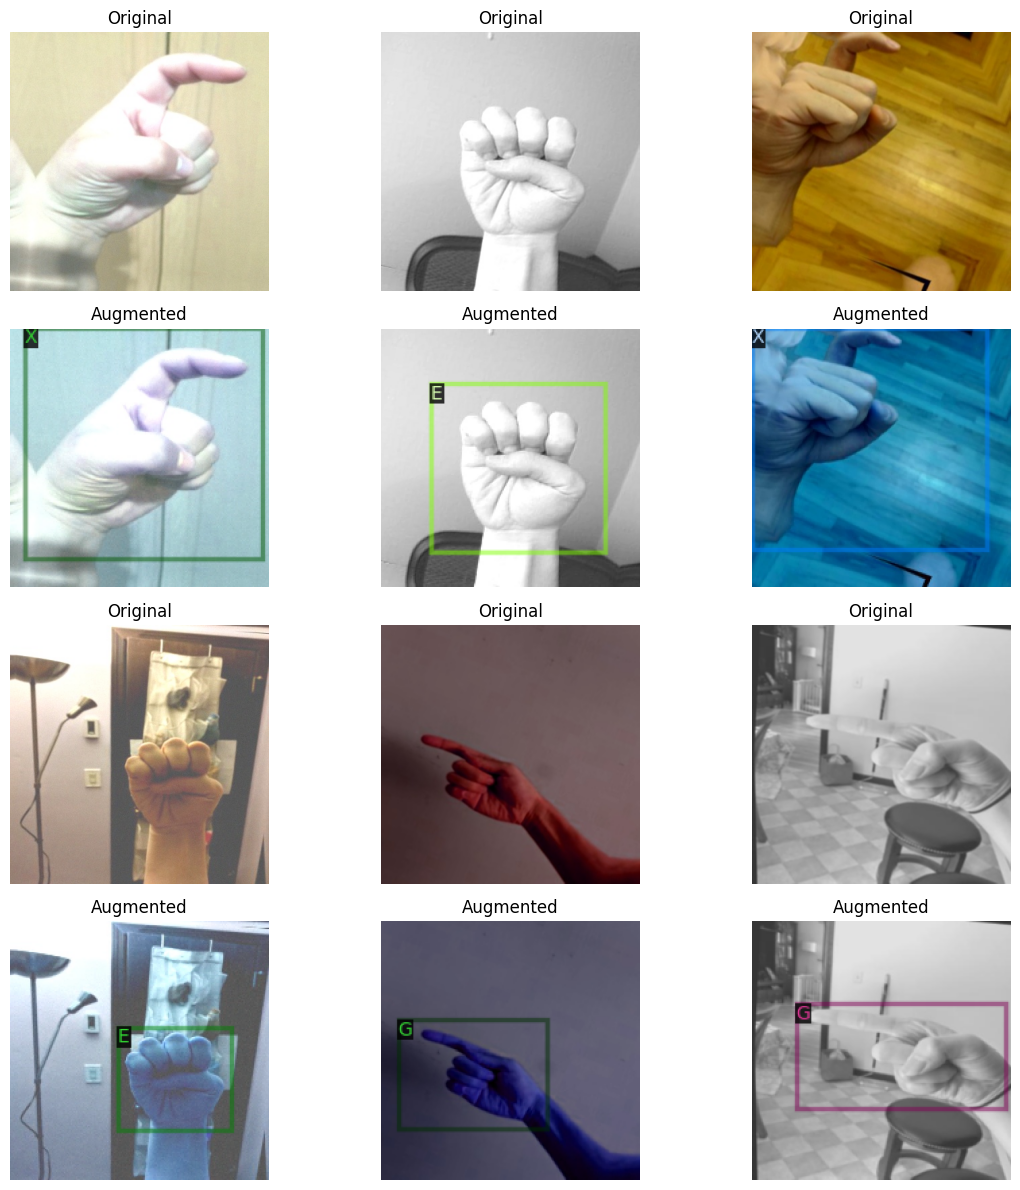
\includegraphics[width=0.7\textwidth]{./images/data_pics.png}
    \caption{Original and Augmented Images}
    \label{fig:Images}
\end{figure}

\newpage
\section{Experiment Settings}
\subsection{Models Used}
\begin{itemize}
    \item \textbf{YOLOv11\cite{2, 7}:} YOLOv11 employs the Ultralytics package for implementation and offers three variants (n, l, x) with different sizes and computational complexities. It introduces spatial attention mechanisms and multi-scale detection layers for enhanced performance, particularly in cluttered scenes.
    \begin{figure}[htbp]
        \centering
        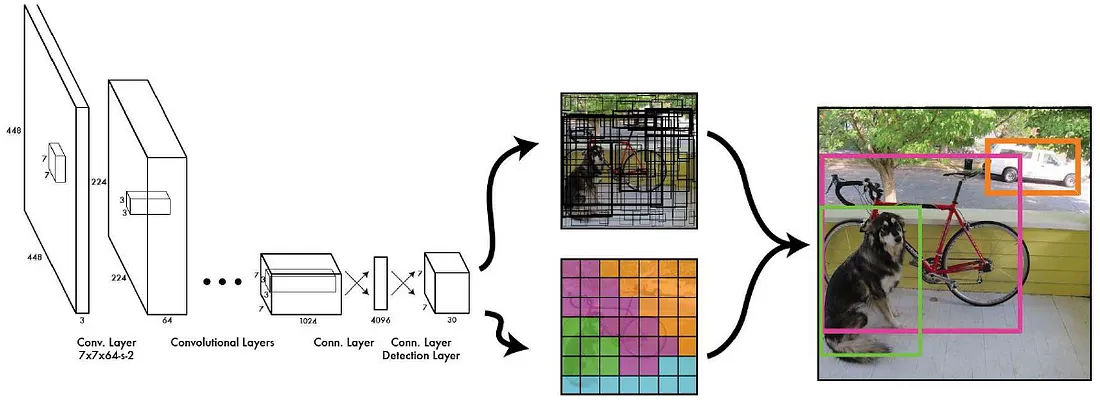
\includegraphics[width=0.6\textwidth]{./images/yolo_arch.png}
        \caption{YOLO Architecture}
        \label{fig:Images}
    \end{figure}
    \item \textbf{Faster R-CNN\cite{4, 6}:} Using the Detectron2 package, Faster R-CNN follows a two-stage detection architecture with a Region Proposal Network (RPN) for generating proposals. It includes a classification head and bounding box regressor. This model uses ResNet or VGG backbones.
    \begin{figure}[htbp]
        \centering
        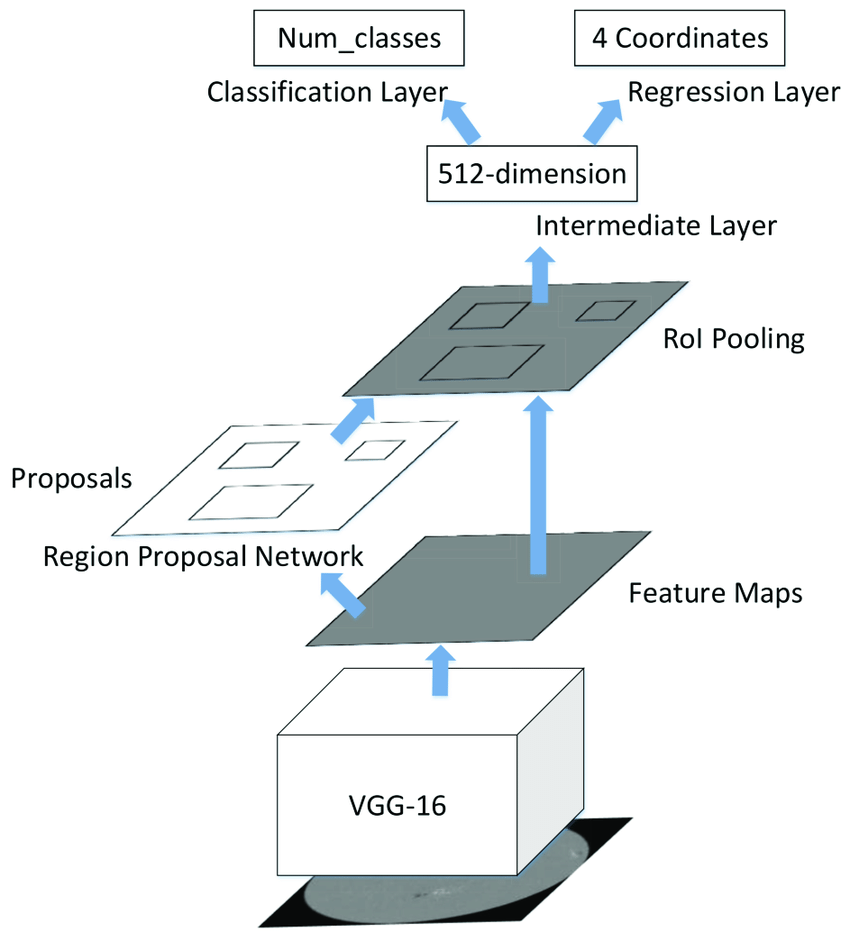
\includegraphics[width=0.6\textwidth]{./images/faster_rcnn_arch.png}
        \caption{Faster RCNN Architecture}
        \label{fig:Images}
    \end{figure}
    \item \textbf{RT-DETR\cite{3, 7}:} RT-DETR is implemented using the Ultralytics package and offers two size variants. It leverages an encoder-decoder structure with hybrid feature extraction, enhancing object detection through attention-based intra-scale interactions and cross-scale fusion.
    \begin{figure}[htbp]
        \centering
        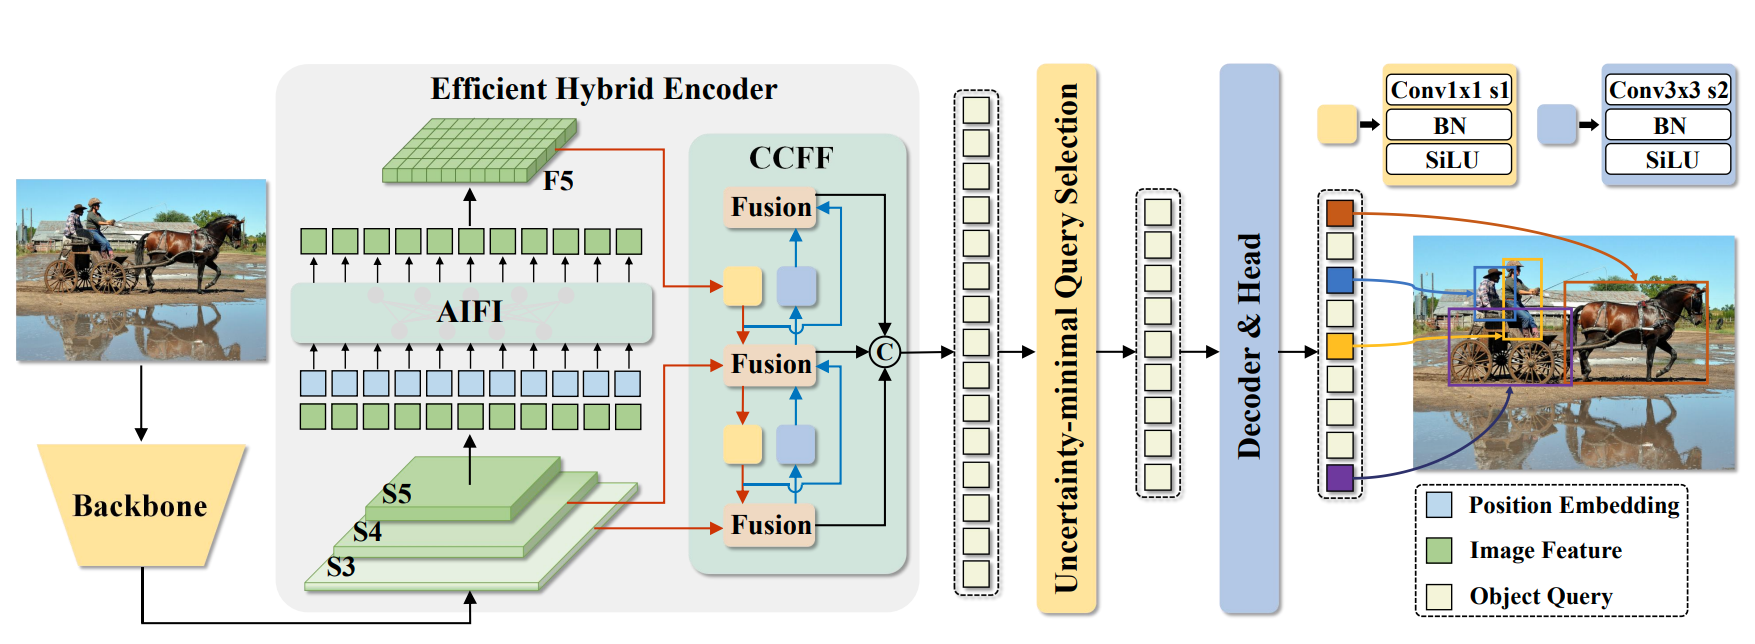
\includegraphics[width=1.0\textwidth]{./images/rt_detr_arch.png}
        \caption{RT-DETR Architecture}
        \label{fig:Images}
    \end{figure}
\end{itemize}
All the model used are pretrained on COCO\cite{8} dataset in order to give a fair comparison.


\subsection{Training Setup}
Models were trained on GPUs with configurations based on memory requirements and optimized using the AdamW optimizer\cite{9} for 15 epochs:
\begin{itemize}
    \item \textbf{YOLOv11-n, YOLOv11-l, Faster R-CNN, RT-DETR-l:} 8GB GPU.
    \item \textbf{YOLOv11-x, RT-DETR-x:} RTX-6000 GPU with 48GB memory.
\end{itemize}

\subsection{Evaluation Metrics}
\begin{itemize}
    \item \textbf{Average Precision (AP):} 
    \[
    \text{AP} = \int_0^1 P(r) \, dr, \quad \text{or} \quad 
    \text{AP} = \frac{1}{n} \sum_{i=1}^{n} P(i),
    \]
    where \( P(r) \) is precision as a function of recall, and \( n \) is the number of recall levels when using the interpolation method.

    \item \textbf{Mean Average Precision (mAP):} 
    \[
    \text{mAP} = \frac{1}{N} \sum_{c=1}^{N} \text{AP}_c,
    \]
    where \( N \) is the number of classes.

    \item \textbf{Intersection over Union (IoU):} 
    \[
    \text{IoU} = \frac{\text{Area of Overlap}}{\text{Area of Union}}
    \]

    \item \textbf{Mean Average Precision 50 (mAP 50):} 
    \[
    \text{mAP 50} = \frac{1}{N} \sum_{c=1}^{N} \text{AP}_c \, \text{ (IoU threshold = 0.50)}.
    \]

    \item \textbf{Mean Average Precision 50-95 (mAP 50-95):} 
    \[
    \text{mAP 50-95} = \frac{1}{N} \sum_{c=1}^{N} \frac{1}{T} \sum_{t=1}^{T} \text{AP}_{c,t},
    \]
    where \( T \) is the total number of IoU thresholds, thresholds = [0.50, 0.55, ..., 0.95].
\end{itemize}

\subsection{Loss Functions}
\paragraph{Faster R-CNN Loss:}
The total loss for Faster R-CNN is:
\[
L_{\text{Faster R-CNN}} = L_{\text{RPN}} + L_{\text{Detection}}
\]
where:
\begin{itemize}
    \item \( L_{\text{RPN}} \): Region Proposal Network loss, combining classification and regression losses.
    \item \( L_{\text{Detection}} \): Detection loss for refining proposals.
\end{itemize}
The Region Proposal Network (RPN) loss combines classification and regression components to generate region proposals:
\[
L_{\text{RPN}} = \frac{1}{N_{\text{cls}}} \sum_{i} L_{\text{cls}}^{\text{RPN}}(p_i, p_i^*) + \lambda \frac{1}{N_{\text{reg}}} \sum_{i} \mathbf{1}_{i}^{\text{obj}} L_{\text{reg}}(t_i, t_i^*)
\]
where:
\begin{itemize}
    \item \( L_{\text{cls}}^{\text{RPN}}(p_i, p_i^*) \): Binary classification loss for objectness:
    \[
    L_{\text{cls}}^{\text{RPN}}(p_i, p_i^*) = - \Big[ p_i^* \log p_i + (1 - p_i^*) \log (1 - p_i) \Big]
    \]
    \item \( L_{\text{reg}}(t_i, t_i^*) \): Smooth L1 loss for bounding box regression.
    \item \( p_i^* \): Ground truth objectness label (1 for object, 0 for background).
    \item \( t_i, t_i^* \): Predicted and ground truth bounding box coordinates.
    \item \( N_{\text{cls}}, N_{\text{reg}} \): Normalization factors for classification and regression losses.
    \item \( \lambda \): Balancing weight for the two losses.
\end{itemize}

The detection loss combines classification and regression losses for proposals refined by the RPN:
\[
L_{\text{Detection}} = \frac{1}{N} \sum_{i} L_{\text{cls}}(p_i, p_i^*) + \lambda \frac{1}{N} \sum_{i} \mathbf{1}_{i}^{\text{obj}} L_{\text{reg}}(t_i, t_i^*)
\]

\paragraph{YOLO Loss:}
The YOLO loss function combines:
\[
L_{\text{YOLO}} = \lambda_{\text{box}} L_{\text{box}} + \lambda_{\text{obj}} L_{\text{obj}} + \lambda_{\text{cls}} L_{\text{cls}}
\]
where:
\begin{itemize}
    \item \( L_{\text{box}} \): Complete IoU (CIoU) loss for bounding box regression.
    \item \( L_{\text{obj}} \): Binary cross-entropy loss for objectness.
    \item \( L_{\text{cls}} \): Cross-entropy loss for classification.
\end{itemize}
The Complete IoU (CIoU) loss improves bounding box regression by considering the geometric factors of overlap, center distance, and aspect ratio:
\[
\text{CIoU} = 1 - \text{IoU} + \frac{\rho^2(b, b^*)}{c^2} + \alpha v
\]
where:
\begin{itemize}
    \item \( \rho(b, b^*) \): Center distance between the predicted and ground truth boxes.
    \item \( c \): Diagonal of the smallest enclosing box covering the predicted and ground truth boxes.
    \item \( v \): Aspect ratio consistency.
    \item \( \alpha \): Weight for the aspect ratio term.
\end{itemize}

\paragraph{RT-DETR Loss:}
The loss function for RT-DETR is:
\[
L_{\text{RT-DETR}} = \lambda_{\text{cls}} L_{\text{cls}} + \lambda_{\text{L1}} L_{\text{L1}} + \lambda_{\text{GIoU}} L_{\text{GIoU}}
\]
where:
\begin{itemize}
    \item \( L_{\text{cls}} \): Cross-entropy loss for classification.
    \item \( L_{\text{L1}} \): L1 loss for bounding box regression.
    \item \( L_{\text{GIoU}} \): Generalized IoU loss for bounding box refinement.
\end{itemize}
The Generalized IoU (GIoU) loss refines bounding box regression by penalizing non-overlapping regions:
\[
L_{\text{GIoU}} = 1 - \text{IoU} + \frac{|C - (A \cup B)|}{|C|}
\]
where:
\begin{itemize}
    \item \( \text{IoU} \): Intersection over Union between predicted and ground truth boxes.
    \item \( C \): Area of the smallest enclosing box covering both the predicted and ground truth boxes.
    \item \( A \): Area of the predicted box.
    \item \( B \): Area of the ground truth box.
\end{itemize}

\subsection{Training and Validation Plot}
    \begin{figure}[htbp]
        \centering
        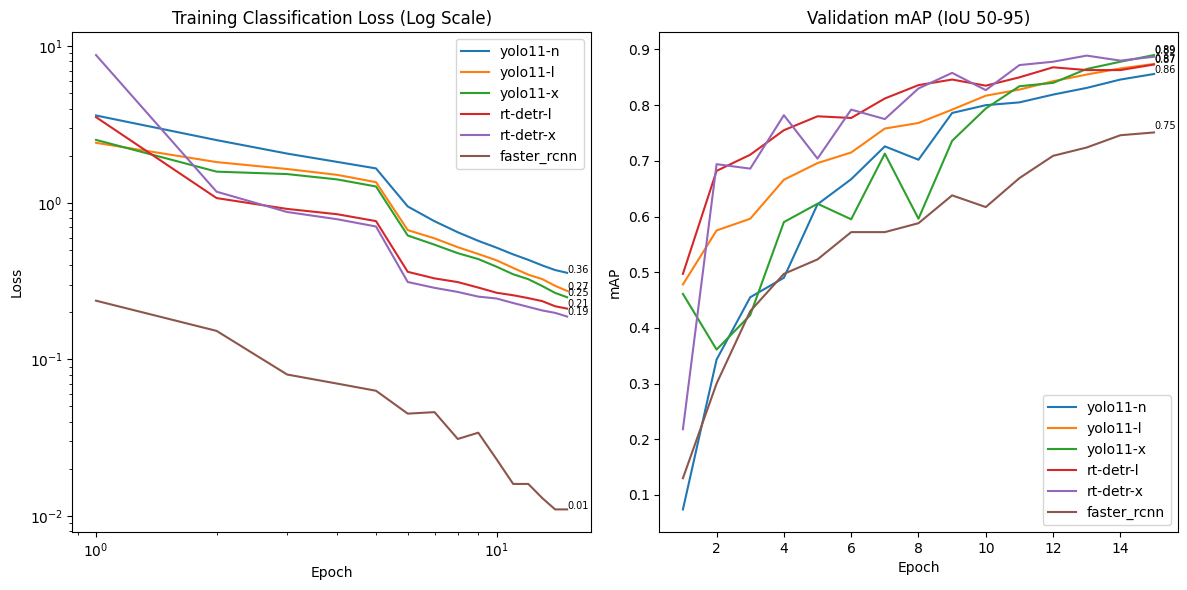
\includegraphics[width=1.0\textwidth]{./images/training.png}
        \caption{Training Loss and Validation mAP50-95}
        \label{fig:Images}
    \end{figure}


\newpage
\section{Results and Discussion}
\begin{table}[h!]
    \centering
    \begin{tabular}{|l|c|c|c|c|}
    \hline
    Model & Latency (ms) & mAP 50-95 & Params (M) & Training Time (s) \\
    \hline
    YOLOv11-n & \textbf{3.32} & 0.692 & \textbf{2.5} & \textbf{160} \\
    YOLOv11-l & 7.49 & 0.777 & 25.3 & 170 \\
    YOLOv11-x & 13.85 & 0.778 & 56.9 & \textbf{140} \\
    RT-DETR-l & 9.5 & 0.753 & 32.9 & 400 \\
    RT-DETR-x & 14.4 & \textbf{0.793} & 67.4 & 215 \\
    Faster R-CNN & 20.69 & 0.555 & 32.3 & 440 \\
    \hline
    \end{tabular}
    \caption{Performance comparison of object detection models.}
    \label{tab:performance_metrics}
\end{table}

The results in Table \ref{tab:performance_metrics} highlight key trade-offs between latency, accuracy, and computational complexity among the evaluated models:
\begin{itemize}
    \item \textbf{YOLOv11:} The smaller variant (YOLOv11-n) offers the fastest inference time but at the cost of some reduced accuracy. The larger variant (YOLOv11-x) achieves a higher mAP but requires more computational resources. 
    However the Average training and inference time in same scale is the fastest among the tested models.
    \item \textbf{RT-DETR:} The medium-sized model (RT-DETR-l) strikes a balance between accuracy and latency, while the larger model (RT-DETR-x) provides the best mAP among all models tested.
    \item \textbf{Faster R-CNN:} While mAP 50-95 is the lowest among the tested models, Faster R-CNN also exhibits the longest latency and highest training time due to its two-stage detection architecture.
\end{itemize}

\begin{figure}[htbp]
    \centering
    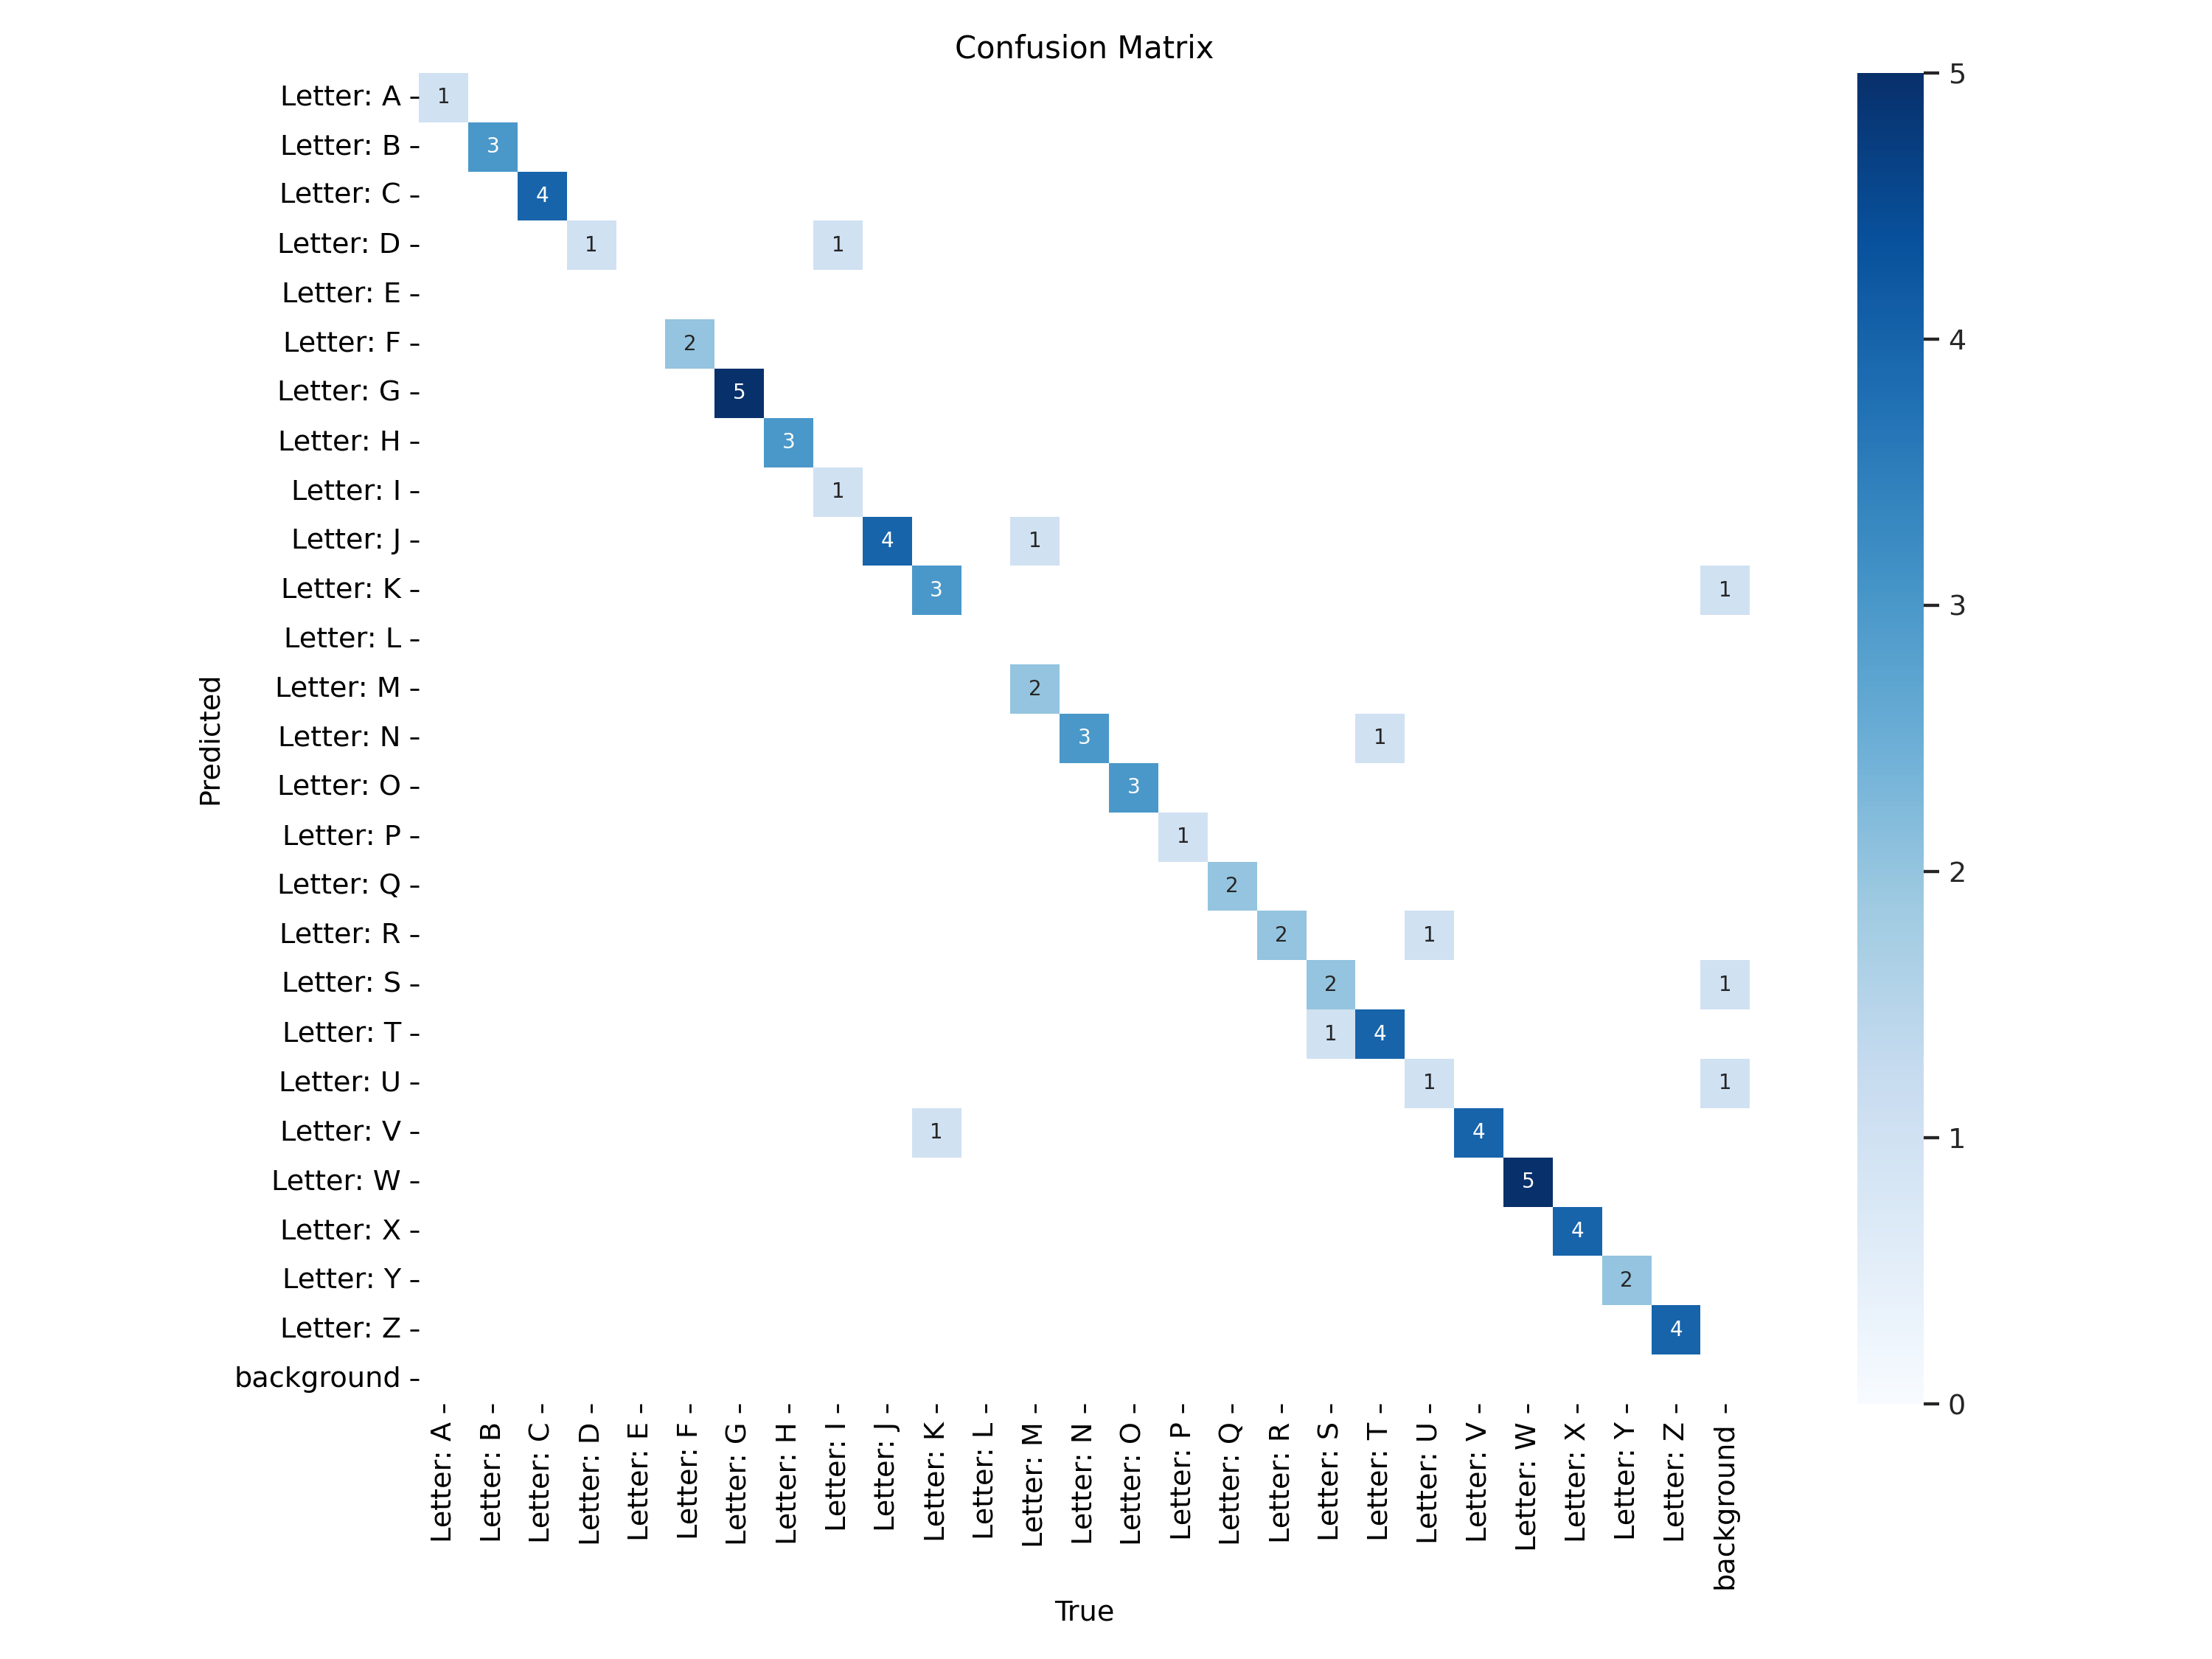
\includegraphics[width=0.6\textwidth]{./images/confusion_matrix.png}
    \caption{YOLOv11-l Confusion Matrix on test data}
    \label{fig:Images}
\end{figure}


\subsection{Error Analysis}
The left picture grid represents the ground truth, and the right picture grid shows the model predictions.
In this batch, the center image was misclassified (I to D). In the left grid (ground truth), the row 2, column 2 position represents the letter "I," while the corresponding image in the right grid (predictions) is classified as "D."
Although the distinction between these letters is clear to humans ("I" involves a pointed pinky finger, while "D" features a pointed index finger), the model seems unable to differentiate between the front and back of the hand. 
This could be due to the overall shape of the "D" being more dominant in the model's learned features. The confidence level for this prediction is only 0.6, reflecting the model's uncertainty.
This analysis suggests that the model might benefit from additional training samples emphasizing hand orientation and finer-grained details, especially for visually similar letters.
\begin{figure}[h!]
    \centering
    \begin{minipage}[b]{0.45\textwidth}
        \centering
        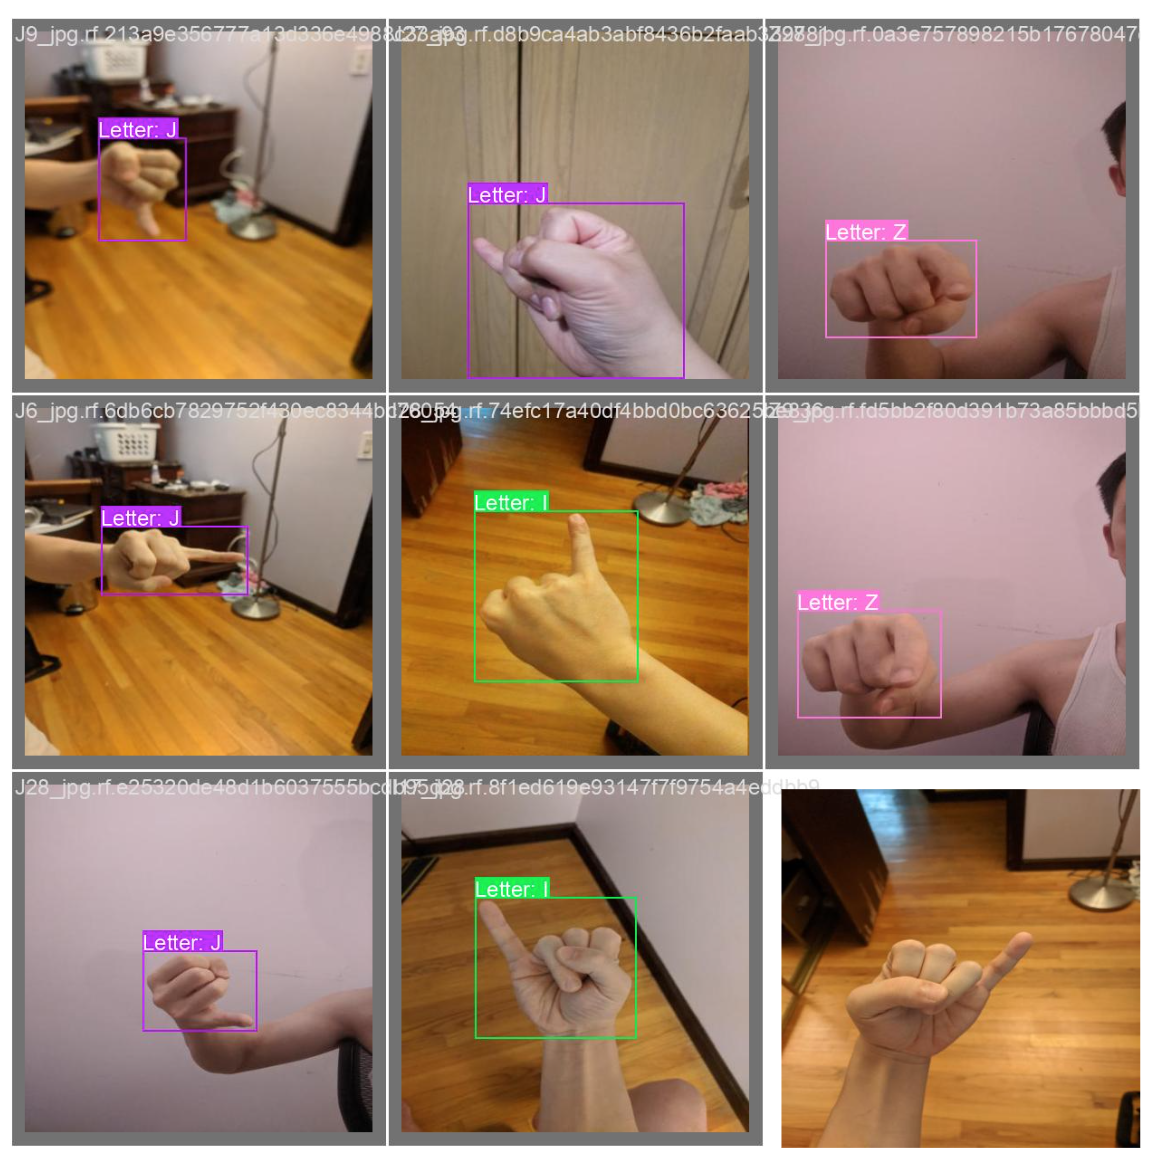
\includegraphics[width=\textwidth]{./images/test_labels.png}
        % \subcaption{Ground Truth}
    \end{minipage}
    \hfill
    \begin{minipage}[b]{0.45\textwidth}
        \centering
        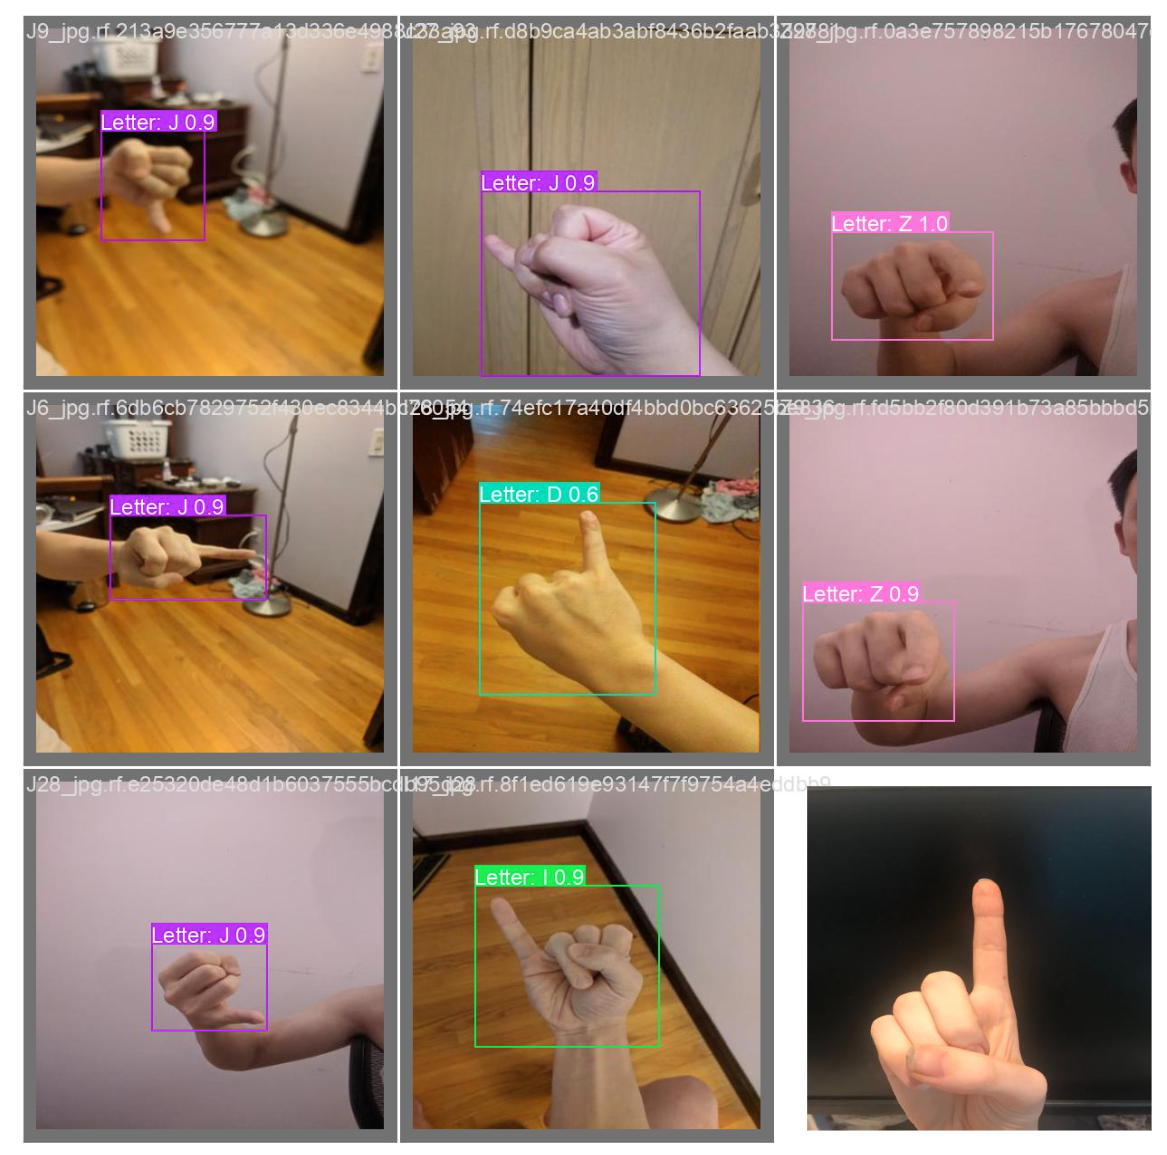
\includegraphics[width=\textwidth]{./images/test_predicts.png}
        % \subcaption{Predicted Output}
    \end{minipage}
    \caption{Comparison of ground truth (left) and predicted output (right) grids.}
    \label{fig:error_analysis}
\end{figure}

\newpage
\section{Conclusion and future work}
This project demonstrates the efficacy of advanced object detection models for American Sign Language (ASL) gesture recognition. 
The evaluation of models highlighted the strengths and trade-offs associated with each approach.
Among the models evaluated, YOLOv11-l emerged as a highly reliable option due to its balance of accuracy, latency, and parameter efficiency. 
Its performance demonstrates that a pretrained YOLOv11-l model is an excellent choice for tasks requiring a balance of speed and accuracy without the need for high computational resources.
RT-DETR-x provided the best overall mAP 50-95, showcasing its potential as a state-of-the-art detection model. With its encoder-decoder structure and attention mechanisms, 
RT-DETR-x is well-suited for handling complex object detection scenarios (not shown in this project due to training data). Although it requires more computational resources, its superior accuracy makes it a highly promising model for future applications.
Future work will focus on incorporating multimodal approaches and more complicated dataset, such as integrating hand tracking with gesture recognition, to improve model robustness and dataset beyond hand sign language with more overlapped different sized objects in one image. 
Additionally, enhancing real-time capabilities, particularly for high-performing models like RT-DETR-x, will be explored to address practical deployment challenges in current systems. \\

    Also, there are some letters such as letter j and z in the ASL dataset are continous frames (involve hand movements), how to detect and understand those letters remains undone. In current dataset it is just simply letters, but if we accpet continous frames as input and 
aim to detect it, it is called \textbf{Spatio-Temporal Action Localization}\cite{10}, which is a potentially important computer vision taksk in the future.\\

The code, data and writings are uploaded to google drive at \url{https://drive.google.com/drive/folders/1ponMZ5jPrbrSf1A7PvU9hFxSyjd909EF}.
The code, writings are also uploaded to github at \url{https://github.com/BigMasonFang/ASL-detection}

\bibliographystyle{plain}
\bibliography{references}
\end{document}
